\documentclass[a4paper, 12pt]{article}
\usepackage[english]{babel}
\usepackage[utf8]{inputenc}
\usepackage[T1]{fontenc}
\usepackage{lmodern}
\usepackage{hyperref}
\usepackage[numbers, sort&compress]{natbib}
\usepackage{calc}
\usepackage{fancyhdr}
\usepackage{graphics}
\usepackage{nowidow}
\usepackage{color}
\usepackage{subcaption}
\usepackage{enumitem}
\usepackage{epsfig}
\usepackage{epstopdf}
\usepackage{verbatim}
\usepackage{listings}

% Matlab colors
\definecolor{dkgreen}{rgb}{0,0.6,0}
\definecolor{gray}{rgb}{0.5,0.5,0.5}
\definecolor{mauve}{rgb}{0.58,0,0.82}
 
% Listings settings
\lstset{ %
  language=Matlab,                % the language of the code
  basicstyle=\footnotesize\ttfamily, % the size of the fonts that are used for the code
  numbers=left,                   % where to put the line-numbers
  numberstyle=\scriptsize\ttfamily\color{gray},  % the style that is used for the line-numbers
  stepnumber=1,                   % the step between two line-numbers. If it's 1, each line 
                                  % will be numbered
  numbersep=10pt,                 % how far the line-numbers are from the code
  showspaces=false,               % show spaces adding particular underscores
  showstringspaces=false,         % underline spaces within strings
  showtabs=false,                 % show tabs within strings adding particular underscores
  tabsize=4,                      % sets default tabsize to 2 spaces
  breaklines=true,                % sets automatic line breaking
  breakatwhitespace=true,         % sets if automatic breaks should only happen at whitespace
  keywordstyle=\color{blue},      % keyword style
  commentstyle=\color{dkgreen},   % comment style
  stringstyle=\color{mauve},      % string literal style
  escapeinside={\%*}{*)},         % if you want to add a comment within your code
  morekeywords={*,...}            % if you want to add more keywords to the set
}


\newlength{\oneLine}
\setlength{\oneLine}{12pt}

\newlength{\eqMargin}
\newlength{\eqHorizMargin}
\newlength{\eqVertMargin}

\setlength{\eqMargin}{20mm}
\setlength{\eqHorizMargin}{\eqMargin}
\setlength{\eqVertMargin}{\eqMargin}

% Paper
\setlength{\paperwidth}{210mm}
\setlength{\paperheight}{297mm}

% Rid the extra space
\setlength{\hoffset}{-1in}
\setlength{\voffset}{-1in}
\addtolength{\hoffset}{\eqHorizMargin}
\addtolength{\voffset}{\eqVertMargin}

% Set margin from the page border (horizontal)
\setlength{\oddsidemargin}{0pt}
\setlength{\evensidemargin}{0pt}

% Header
\setlength{\topmargin}{0pt}
\setlength{\headheight}{42pt}
\setlength{\headsep}{18pt}
\renewcommand{\headrulewidth}{0pt}

% Footer
\addtolength{\footskip}{18pt}
\renewcommand{\footrulewidth}{0pt}

% Margin notes
\setlength{\marginparsep}{0pt}
\setlength{\marginparwidth}{0pt}

% Text
\setlength{\textwidth}{\paperwidth - \hoffset - \hoffset - 25.4mm - 25.4mm}
\setlength{\textheight}{\paperheight - \voffset - \topmargin - \headheight - \headsep - \footskip - \voffset - 25.4mm - 25.4mm}

%\setlength{\labelwidth}{20mm}

% Hyperref settings
\hypersetup{
    unicode=true,					% non-Latin characters in Acrobat's bookmarks
    pdftoolbar=true,				% show Acrobat's toolbar?
    pdfmenubar=true,				% show Acrobat's menu?
    pdffitwindow=false,				% window fit to page when opened
    pdfstartview={FitH},			% fits the width of the page to the window
    pdftitle={S-26.3120 Radio Engineering, laboratory course},	% title
    pdfauthor={Tuomas Leinonen} {Francisco Solano Eizaguirre} {Mikko Heino},	% author
    pdfsubject={Radio Engineering},	% subject of the document
    pdfcreator={LaTeX},				% creator of the document
    pdfproducer={Aalto},			% producer of the document
    pdfkeywords={radio} {antenna} {measurement},	% list of keywords
    pdfnewwindow=true,				% links in new window
    colorlinks=true,				% false: boxed links; true: colored links
    linkcolor=black,				% color of internal links
    citecolor=black,				% color of links to bibliography
    filecolor=black,				% color of file links
    urlcolor=black					% color of external links
}

% Bad hyphenation
%\hyphenation{}

% Macros
\newcommand{\dB}{\mathrm{\;dB}}
\newcommand{\dBm}{\mathrm{\;dBm}}
\newcommand{\m}[1]{\mathrm{#1}}

\newcommand\varpm{\mathbin{\vcenter{\hbox{%
  \oalign{\hfil$\scriptstyle+$\hfil\cr
          \noalign{\kern-.3ex}
          $\scriptscriptstyle({-})$\cr}%
}}}}
\newcommand\varmp{\mathbin{\vcenter{\hbox{%
  \oalign{$\scriptstyle({+})$\cr
          \noalign{\kern-.3ex}
          \hfil$\scriptscriptstyle-$\hfil\cr}%
}}}}

\definecolor{dkred}{rgb}{0.6, 0, 0}
\definecolor{dkgrn}{rgb}{0, 0.6, 0}
\definecolor{dkblue}{rgb}{0, 0, 0.6}
\definecolor{gray}{rgb}{0.8, 0.8, 0.8}

\pagestyle{fancy}
\lhead{S-26.3120 Radio Engineering, laboratory course\\Lab 4: Amplifier -- Pre-study Report}
\rhead{Tuomas Leinonen, 84695P\\}
\cfoot{\thepage}


\begin{document}

\begin{titlepage}
\pagestyle{empty}
\begin{center}

\vspace*{30mm}
\noindent\LARGE{\textbf{S-26.3120 Radio Engineering, laboratory course}}

\vspace*{20mm}

\Large{\textbf{Lab 4: Amplifier}}\\

\vspace*{15mm}

\large{\textbf{Pre-study Report}}\\
\vspace{15mm}
\large{\today}
	
\vspace*{30mm}
\large{Tuomas Leinonen, 84695P, Group 1}

\end{center}

\end{titlepage}

\section{Theoretical background}

\textit{Answer the following questions briefly.}

\vspace*{0.5\oneLine}
\noindent
For more thorough discussions, the reader is encouraged to get acquainted with 
the reference material listed at the end of this document.

\subsection{Describe the procedure to design a low-noise microwave transistor amplifier.}

First of all, one needs some ``goals''; a set specifications to be fulfilled. These are 
given (like in our labs) or derived from the system specifications when other blocks are 
taken into account. These are usually given in terms of (stability), power gain, bandwidth 
and noise; along with physical properties of the application and/or usage environment 
(temperature, size, price/cost and biasing/power constrictions, for example).

Next, the PCB-material and transistor(s) and its (their) configuration, including DC biasing, 
is selected carefully based on specifications. It is best to go for the simplest design that 
meets the requirements by a suitable margin. After this, transistor loading is determined. 
That is, the source and load reflection coefficients (i.e., the matching circuits, 
see question 1.5) yielding wanted properties (listed in the previous paragraph) are 
found. For this, one commonly uses hand calculation with $S$-parameters, Smith-charts 
and possibly Matlab, or circuit simulators along with other CAD-tools.

Now that we have the ``ideal'' design, we use a RF-simulator, such as ADS, to design the 
actual amplifier layout. This icludes the biasing and matching circuits as accurately 
as possible. The design is then rigorously simulated, tweaking the circuit until optimum 
performance is achieved. One should take practical limitations into account in this phase.

The amplifier is then manufactured and measured in real-life. If the specifications are 
not met, designers must seek to discover the source of the problem. Fixing the problem may 
require some tweaking in the already manufactured product or a complete redesign depending 
on its severity. Careful layout design and rigorous simulation will help to avoid such 
situations.


\subsection{Describe the various methods by which the amplifier can be stabilized. 
	What are the tradeoffs when using different methods to stabilize the transistor?}
\label{s:ts}

Using the two-port approach, an amplifier may oscillate when the either of its ports, 
input or output, presents a negative resistance. This corresponds to a situation where 
$|\rho_\mathrm{in}| > 1$ or $|\rho_\mathrm{out}| > 1$. Thus to stabilize a resistor, 
these are to be made less than unity. One should note that said reflection coefficients 
are dependent on input and source loading (i.e., $\rho_\mathrm{in} > 1$ and $\rho_\mathrm{L}$), 
and that stability is frequency dependent due to its $S$-parameters being a function 
of frequency. Thus the designer needs to confirm that the circuit is stable at all 
frequencies.

This may be achieved by atleast two means; by resistive loading or by adding negative 
feedback. Both of these methods are mainly used for stabilizing broadband amplifiers, 
and the stability of narrowband amplifiers is ensured by a careful selection of source 
and load reflection coefficients. This is because all of the aforementioned stabilization 
techniques have negative effect on gain, noise and/or $\mathit{VSWR}$ performance of the
amplifier. Especially resistive loading at source has a drastic effect on noise performance. 
On the other hand, stabilizations methods may in some cases be used to meet design goals.


\subsection{What is the difference between the unilateral and bilateral scenario in 
	designing transistor amplifiers	and how does it impact the design? 
	What is the unilateral figure of merit?}

A two-port is said to be unilateral (``one-directional'') if and only if its $S_{12} = 0$. 
Otherwise the two-port in question is bilateral (``two-directional''), and bilateral design 
routine must be used. While bilateral design techniques may be used always, unilateral 
techniques are easier than their bilateral counterparts. This is due to the source and load 
reflection coefficients being independent of each other and may thus be designed separately. 
The loading of bilateral amplifiers is rather complicated since both source and load 
matching ($\rho_\mathrm{in}$ and $\rho_\mathrm{out}$, respectively) are cross-dependent. 
This may be seen in the definition of said reflection coefficients:
\begin{eqnarray}
\rho_\mathrm{in} & = & S_{11} + \frac{S_{12} S_{21} \rho_\mathrm{L}}{1 - S_{22} \rho_\mathrm{L}} 
	\;\;=\;\; S_{11} \textrm{, when } S_{12} = 0, \label{e:rhoin} \\ 
\rho_\mathrm{out} & = & S_{22} + \frac{S_{12} S_{21} \rho_\mathrm{S}}{1 - S_{11} \rho_\mathrm{S}}
	\;\;=\;\; S_{22} \textrm{, when } S_{12} = 0. \label{e:rhoout}
\end{eqnarray}

Because of this, most textbooks (like \cite{pozar}) present ``advanced'' design 
procedures, like constant gain and noise circles, only of the unilater case. Luckily a 
bilateral amplifier can be designed using the unilateral methods if its $|S_{12}|$ is 
negligibly small. The validity of this $S_{12} \approx 0$ approximation may be evaluated 
by calculating \textit{the unilateral figure of merit} $U$ for the amplifier in question. 
It is defined as follows:
\begin{equation}\label{e:U}
U = \frac{|S_{11}| |S_{12}| |S_{21}| |S_{2}|}{(1 - |S_{11}|^2)(1 - |S_{22}|^2)}.
\end{equation}

When designing amplifier of maximum gain using (simultaneous) conjugate matching, maximum 
transducer power gain error caused by unilateral approach $G_\mathrm{T} / G_\mathrm{TU}$ 
is given as
\begin{equation}\label{e:U2}
\frac{1}{(1+U)^2} < \frac{G_\mathrm{T}}{G_\mathrm{TU}} < \frac{1}{(1-U)^2}.
\end{equation}
Depending on the specifications, an error of few tenths of a decibel usually justifies 
the use of unilateral design procedure.


\subsection{What is the difference between the operating and available pow\-er gain circles? 
	Which of these should be considered for designing an LNA?}

In literature, one may find three different power gain definitions for a two-port. In 
\cite{pozar} they are defined as follows (one should note that different authors use 
slightly different, yet still a tad confusing, naming convention):
\begin{itemize} \itemsep 0pt
\item Operating power gain $G_\mathrm{P}$, shown in Eq.~(\ref{e:Gp}), is the ratio of 
	power dissipated in the load $Z_\mathrm{L}$ to the power delivered to the input 
	of the two-port network. This gain is independent of $Z_\mathrm{S}$, although the 
	characteristics of some active devices may be dependent on $Z_\mathrm{S}$.

\item Available power gain $G_\mathrm{A}$, shown in Eq.~(\ref{e:Ga}), is the ratio of the 
	power available from the two-port network to the power available from the source. 
	This assumes conjugate matching of both the source and the load, and depends on 
	$Z_\mathrm{S}$, but not $Z_\mathrm{L}$.

\item Transducer power gain $G_\mathrm{T}$, shown in Eq.~(\ref{e:Gt}), is the ratio of 
	the power delivered to the load to the power available from the source. This depends 
	on both $Z_\mathrm{S}$ and $Z_\mathrm{L}$.
\end{itemize}
While transducer gain is the most useful in general, we need to compare the first two to 
each other in this task.
\begin{eqnarray}
G_\m{P} \;\;=& \displaystyle \frac{P_\m{L}}{P_\m{in}} 		&=\;\; \frac{|S_{21}|^2 (1 - |\rho_\m{L}|^2)}{(1 - |\rho_\m{in}|^2)|1 - S_{22}\rho_\m{L}|^2} 									\label{e:Gp} \\
G_\m{A} \;\;=& \displaystyle \frac{P_\m{avn}}{P_\m{avs}} 	&=\;\; \frac{|S_{21}|^2 (1 - |\rho_\m{S}|^2)}{|1 - S_{11}\rho_\m{S}|^2 (1 - |\rho_\m{out}|^2)} 							\label{e:Ga} \\
G_\m{T} \;\;=& \displaystyle \frac{P_\m{L}}{P_\m{avs}} 		&=\;\; \frac{|S_{21}|^2 (1 - |\rho_\m{S}|^2)(1 - |\rho_\m{L}|^2)}{|1 - \rho_\m{S}\rho_\m{in}|^2 |1 - S_{22}\rho_\m{L}|^2}	\label{e:Gt} 
\end{eqnarray}

Gonzales recommends a procedure based on constant operating power gain for practical 
designs due to its simplicity, saying it's common practice when $S_{12}$ cannot be 
neglected. On the other hand, using $G_\mathrm{A}$ is beneficial since it can be plot 
on the same Smith chart as constant noise circles, both being dependent on $|\rho_\mathrm{S}|$. 
This way one may find a suitable compromise between gain and noise, and is thus more 
suitable for this lab exercise.

Pozar uses only unilateral approach, looking at source and load ``matching gains'' 
separately. Constant noise circles may be plot on the same Smith chart as constant 
source matching gain circles.


\subsection{What are the different types of matching networks that can be used for 
	matching the source and load? Enumerate the advantages/disadvantages of the different methods.}

In general, matching circuits may be divided into two categories: lossy and lossless matching 
circuits. The former method uses attenuators whereas the latter is accomplished using lumped 
inductors and capacitors, or microstrip transmission lines. Most notable pros and cons of
each realization are listed below \cite{bahl}.
\vspace*{\oneLine}

\noindent\textbf{Attenuation:}
\vspace*{-0.5\oneLine}
\begin{description}[font=\rmfamily\mdseries, leftmargin=15mm, style=sameline, align=right, labelsep=5mm, itemsep=-2pt]
	\item[\boldmath$+$\unboldmath]	Inherently wideband
	\item[\boldmath$+$\unboldmath] 	Small size
	\item[\boldmath$-$\unboldmath] 	Lossy and noisy
	\item[\boldmath$-$\unboldmath] 	Cannot realize arbitrary $\rho$ or $Z$
\end{description}

\noindent\textbf{Microstrip:}
\vspace*{-0.5\oneLine}
\begin{description}[font=\rmfamily\mdseries, leftmargin=15mm, style=sameline, align=right, labelsep=5mm, itemsep=-2pt]
	\item[\boldmath$+$\unboldmath]	Well characterized and flexibility in design
	\item[\boldmath$+$\unboldmath] 	Low loss and high performance
	\item[\boldmath$+$\unboldmath] 	Has better harmonic tuning capability for high-efficiency applications
	\item[\boldmath$-$\unboldmath] 	Strong interaction effects between elements and discontinuities in packed design
	\item[\boldmath$-$\unboldmath] 	Large in size even with interactions included
\end{description}

\noindent\textbf{Lumped \boldmath$LC$\unboldmath-network:}
\vspace*{-0.5\oneLine}
\begin{description}[font=\rmfamily\mdseries, leftmargin=15mm, style=sameline, align=right, labelsep=5mm, itemsep=-2pt]
	\item[\boldmath$+$\unboldmath]	Capable of transforming high impedance ratios
	\item[\boldmath$+$\unboldmath] 	Minimum interactions between elements due to small size
	\item[\boldmath$+$\unboldmath] 	Compact in size
	\item[\boldmath$-$\unboldmath] 	Low $Q$, limited DC power handling capability	
	\item[\boldmath$-$\unboldmath] 	Substandard performance due to low $Q$ at the output of a power amplifier in terms of $P_\mathrm{out}$ and $\mathit{PAE}$
\end{description}

$LC$-networks are used at low frequencies by placing one or more series or shunt elemements after 
one another. When using two or less elements, one may find the matching circuit analytically or 
by using a Smith chart. Inductors may also be used for transistor matching when used as degeneration 
elements. IDCS refers to inductively degerated common source, a topology where series inductances 
are placed at gate and source. These interact with the parasitic gate-source capacitance forming 
a resonator.

Microstrips may be used by alternating impedance along the same line 
(e.g., tapering, quarter-wave transformers or so-called ``high/low-$Z_0$ matching''), or by 
using separate (series/)parallel stubs of certain, distance (from load), length and $Z_0$ (e.g., 
single or two-stub matching). One might also combine aforementioned approaches, or use baluns.

For our amplifier design, the microstrip based approaches are recommended. 
The matching circuits of the amplifier may be found simply by using the traditional conjugate-approach 
of the selected method to match $\rho_\mathrm{S}^*$ and $\rho_\mathrm{L}^*$ (looking toward 
source and load, respectively) to $Z_0$.


\subsection{How is the reflection coefficient of the designed amplifier calculated? 
	What is the compromise when designing an amplifier for low-noise and maximum gain operation?}

The input and output reflection coefficients $\rho_\mathrm{in}$ and $\rho_\mathrm{out}$ 
of any two-port are found using Eq. (\ref{e:rhoin}) and (\ref{e:rhoout}), respectively. 
One should note the cross-depency in the bilateral case (i.e., when $|S_{12}| > 0$). 
Source and load reflection coefficients are chosen based on wanted amplifier characteristics 
(i.e., gain, return loss, noise performance, linearity, optimum power and $\mathit{PAE}$), 
that are often contradictory to one another. Here we focus only on gain and noise figure 
of the amplifier.

Using Pozar's terminology/concepts, we may only affect the ``matching gains'' of the 
transistors. These may be set quite freely within certain bounds (enforced by stability 
requirements, for example) using matching circuits to create suitable loading at the 
input and output. The gain due to $G_0 = |S_{21}|^2$ is constant at given frequency 
and used DC-biasing. 

Maximum gain is obtained when simultaneous conjugate matching is used. Now 
$\rho_\mathrm{in} = \rho_\mathrm{S}^*$ and $\rho_\mathrm{out} = \rho_\mathrm{L}^*$, 
and both ``matching gains'' and return losses are maximized. This situation is rather 
easy to achieve in both uni- and bilateral cases, assuming the transistor remains stable. 
The obtained bandiwdth is usually quite limited, though.

Optimal noise performance is obtained by using suitable source mismatch to cancel some 
of the correlated noise. Doing so decreases the source matching gain. The output matching 
has no effect on noise, and may thus be conjugate-matched to achieve higher gain. One 
should note bandwidth requirements here as well.

Long story short: there's a trade-off between maximum gain and optimum noise performance. 
The designed may trade some of the source matching gain in favor for better noise performance.
For this purpose, constant gain and constant noise figure circles are plot on the same 
Smith chart for $\rho_\mathrm{S}$.


\subsection{Briefly discuss the impact of grounding using plated-through holes (PTH) via.}

Most commonly RF field-effect transistors, such as the pHEMT in question, are used in 
common-source (CS) configuration. In this configuration, gate and drain are used as input 
and output nodes, respectively. The source node is connected to signal ground as such or 
a through a so-called degeneration element; a resistor (rare) or an inductor (IDCS).

Using a degeneration element is justified when performance improvements are achieved through 
well-thought design. Careless design may lead to unstable operation, especially at higher 
frequencies due to parasitic effects. In practice, these parasitic $RLC$ are present in 
all connections -- also in this grounding, where $L$ is typically dominant due to high 
operating frequencies. In some cases, the use of plated-through holes (PTH) is a non-negligible 
source of inductance, limiting the size of the ``actual'' degeneration-inductance if used. 
Especially when a thick substrate is used.

Two PTHs per a source connector (two source connections, four PTHs in total) are embedded in 
the provided $S$-parameters to help the design process. They assume certain substrate 
thickness and PTH placement.


\newpage
\section{Calculations}

For this lab assingment, the design goals and other specifications are given in the following 
two tables (Tables \ref{t:p1} and \ref{t:p2}).

\begin{table}[!h]
	\begin{center}
		\caption{Design specifications for Group 1.}
		\label{t:p1}
		\renewcommand{\arraystretch}{1.2}
		\begin{tabular}{lcrl}
			Paramater					& Symbol						& Value		& Unit 	\\
			\hline
			Operating frequency			& $f_\mathrm{op}$				& 2.5		& GHz 	\\
			Drain-to-Source DC-voltage	& $V_\mathrm{DS}$				& 2			& V 	\\
			Drain-to-Source DC-current	& $I_\mathrm{DS}$				& 30		& mA 	\\
			Minimum gain				& $G_\mathrm{min}$				& 13		& dB 	\\
			Maximum noise figure		& $F_\mathrm{max}$				& 0.8		& dB 	\\
			Minimum return loss			& $\mathit{RL}_\mathrm{min}$	& 15		& dB 
		\end{tabular}
	\end{center}
	\vspace{-\oneLine}
\end{table}

\begin{table}[!h]
	\begin{center}
		\caption{Transistor and PCB specifications.}
		\label{t:p2}
		\renewcommand{\arraystretch}{1.2}
		\begin{tabular}{ll}
			Transistor:	& Avago Technologies ATF-35143 (pHEMT) \\
			PCB:		& RT Duroid 5870 ($h = 0.787$~mm, $\epsilon_\m{r} = 2.3$)
		\end{tabular}
	\end{center}
	\vspace{-\oneLine}
\end{table}

All calculations are based on a MATLAB script using only the so-called ``core features'' of MATLAB. 
This rather lengthy script is shown in Appendix A. For more comprehensive study, a real circuit 
simulator with layout capabilities should be used. Such simulations are left for latter part of 
this lab assignment.

\subsection{For the given specifications of operation, calculate the stability factor and draw the input 
and output stability circles. Is the transistor unconditionally stable? If not, propose methods by which the
stability can be improved.}

The stability of the transistor was investigated using provided $S$-parameters over the whole 
frequency range $0.5 \ldots 18$~GHz. Both Rollet's $|\Delta|-K$ test and the $\mu$ test were 
used. The results of the $\mu$ test are shown in Fig.~\ref{f:mu}. The stabilty factors at the 
specified operating frequency of 2.5~GHz were found to be $|\Delta| = 0.419$, $K = 0.474$ and 
$\mu = 0.437$. Using the specified biasing point, the transistor is potentially unstable. 
Unconditional stability is achieved when $|\Delta| < 1$ and $K > 1$, or equivalently when $\mu > 1$.

\begin{figure}[!h]
	\begin{center}
		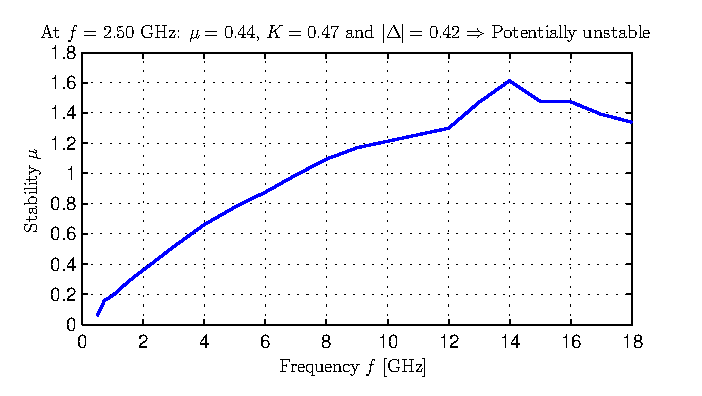
\epsfig{file=img/mu.eps, width=0.6\textwidth}
		\caption{Results from the $\mu$ test: the transistor is unconditionally stable when $f > 7$~GHz.}
		\label{f:mu}
	\end{center}
\end{figure}

For a potentially unstable transitor we may draw input and output stability circles. A two-port 
is stable, when conditions $|\rho_\mathrm{in}| < 1$ and $|\rho_\mathrm{out}| < 1$ are met 
simultaneously using passive loading $|\rho_\mathrm{S,\;L}| < 1$. For unilateral amplifiers, 
these conditions simplify to $|S_{11,\;22}| < 1$.

For bilateral amplifiers, stability circles are drawn for $|\rho_\mathrm{in,\;out}| = 1$ using Eq. 
(\ref{e:CL}-\ref{e:RS}). Output (input) stability circle is a circle with a radius $R_\m{L}$ ($R_\m{S}$), 
centered at $C_\m{L}$ ($C_\m{S}$). Values of $\rho_\m{L}$ ($\rho_\m{S}$) correspond to a situation 
where $|\rho_\mathrm{in}|$ ($|\rho_\mathrm{out}|$) is unity. If $|S_{11,\;22}| < 1$, $|\rho_\mathrm{S,\;L}| = 0$ 
(origin) is in the stable region of the Smith chart. Both input and output stability circles of the
transistor in question are shown in Fig.~\ref{f:SLstab}. The (un)stable regions of the Smith chart 
are also labeled.

\begin{eqnarray}
C_\m{L} &=& \frac{ (S_{22} - \Delta S_{11}^*)^* }{ |S_{22}|^2 - |\Delta|^2 } \qquad \textrm{(center)} \label{e:CL} \\
R_\m{L} &=& \left| \frac{ S_{12} S_{21} }{ |S_{22}|^2 -|\Delta|^2 } \right| \qquad \textrm{(radius)} \label{e:RL} \\
C_\m{S} &=& \frac{ (S_{11} - \Delta S_{22}^*)^* }{ |S_{11}|^2 - |\Delta|^2 } \qquad \textrm{(center)} \label{e:CS} \\
R_\m{S} &=& \left| \frac{ S_{12} S_{21} }{ |S_{11}|^2 -|\Delta|^2 } \right| \qquad \textrm{(radius)} \label{e:RS}
\end{eqnarray}

\begin{figure}[!h]
	\begin{center}
		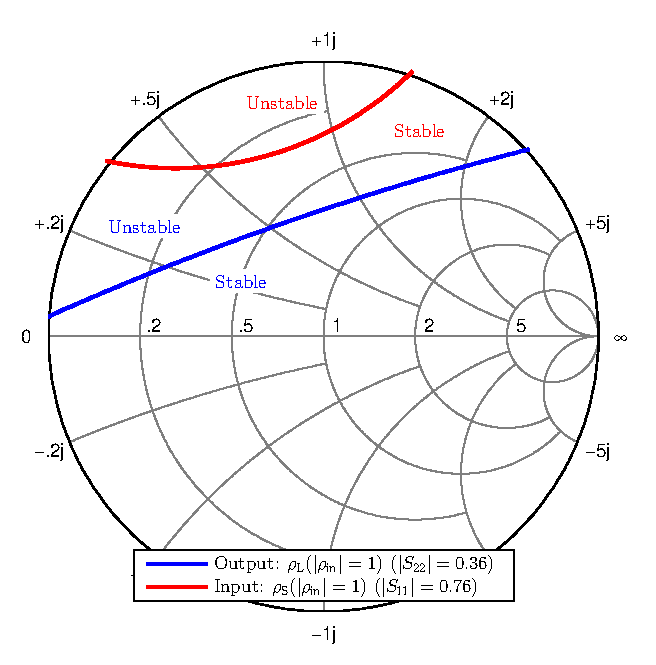
\epsfig{file=img/SLstab.eps, width=0.6\textwidth}
		\caption{Input and output stability circles at $f = 2.5$~GHz.}
		\label{f:SLstab}
	\end{center}
\end{figure}

One might stabilize a potentially unstable amplifier using resistive loading, as was discussed 
in section \ref{s:ts}. There are four ways the resistor may be connected to the amplifier, and 
all of these connections were studied separately. The study were two-fold, conducted using 
transmission parameters derived from provided $S$-parameters. First, resistance values yielding 
unconditionally stable circuit at $f = 2.5$~GHz were determined. These values were processed 
further to determine resistance values capable of meeting specifications. The results of this 
study are shown in Table~\ref{t:s}.

\begin{table}[!h]
	\begin{center}
		\caption{Resistor values needed to achieve unconditional stability and wanted characteristics at $f = 2.5$~GHz.}
		\label{t:s}
		\renewcommand{\arraystretch}{1.2}
		\begin{tabular}{ccccc}
			Port	& Node		& Connection	& $R_\mathrm{uncond.\;stable}$ [$\Omega$]	& $R_\mathrm{spec.\;met}$ [$\Omega$] \\
			\hline
			Input 	& Gate		& Series		& $\geq 15.3$								& Too noisy				\\
			Input 	& Gate		& Shunt			& $\leq 80.9$								& Too noisy				\\
			Output 	& Drain		& Series		& $\geq 37.8$								& $69.8 \ldots 109$ 	\\
			Output  & Drain		& Shunt			& $\leq 6.27$								& Not enough gain		\\
		\end{tabular}
	\end{center}
	\vspace{-\oneLine}
\end{table}

For the rest of this report, the transistor is assumed to be stabilized using a series resistance 
of 100~$\Omega$ connected to the output (drain) of the transistor. This stabilization method and 
the value was selected because it was found to meet all requirements with relatively good margins. 
The value of 100 $\Omega$ is very good choice due to its availability in all standardized resistor 
series (E6$\ldots$192). A more thorough discussion is presented in section \ref{s:gf}.


\subsection{Can you use the unilateral or bilateral scenario for the design of the transistor amplifier? 
Justify your selection.}

The unilateral figure of merit and the gain error resulting from (stabilized) unilateral approach are 
shown in Figures \ref{f:U} and \ref{f:DeltaG}, respectively. At 2.5~GHz, $|S_{12}| = 0.0424$, $U = 0.0967$ 
and $-0.802 < G_\mathrm{T}/G_\mathrm{TU} < +0.884$ [dB]. Due to rather strict design goals, unilateral 
approach is not appropriate. For this reason, bilateral analysis was used. One cannot ``go wrong'' with 
bilateral analysis since it's valid even for truly unilateral designs.

\begin{figure}[!h]
	\begin{center}
		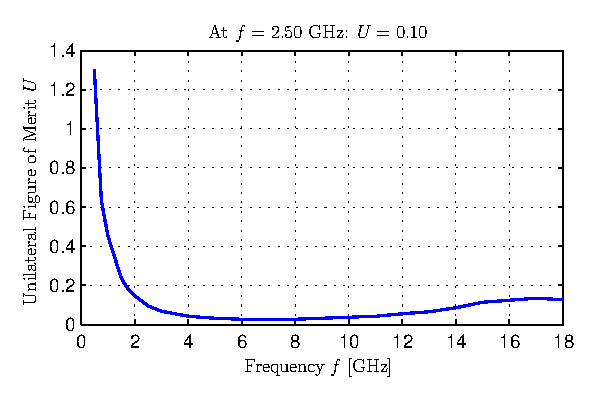
\epsfig{file=img/UFM.eps, width=0.6\textwidth}
		\caption{The unilateral figure of merit $U$ as a function of frequency $f$.}
		\label{f:U}
	\end{center}
\end{figure}

\begin{figure}[!h]
	\begin{center}
		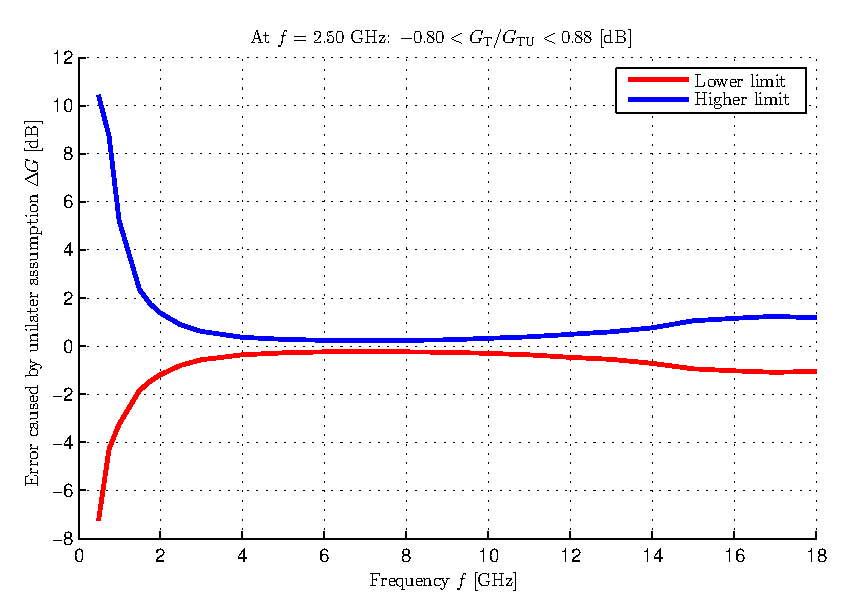
\epsfig{file=img/DeltaG.eps, width=0.6\textwidth}
		\caption{asd}
		\label{f:DeltaG}
	\end{center}
\end{figure}


\newpage
\subsection{Draw the gain and noise circles. Calculate the input and output reflection 
	coefficients and design the matching networks. Does the input reflection coefficient 
	satisfy the requirement? If not, what can be done?}
\label{s:gf}

The constant available gain and noise figure circles of the stabilized transistor are shown 
on the $\rho_\mathrm{S}$ Smith chart in Fig.~\ref{f:GFcirc}, drawn using Eq. (\ref{e:CA}-\ref{e:RF}). 
Smaller circles are for larger $G_\mathrm{A}$s and smaller $F$s. To meet gain and noise figure 
specifications, the source reflection coefficient must be chosen from the area enclosed within 
both $G_\mathrm{A} = 13$~dB and $F = 0.8$~dB circles (both dashed). One may think of it as a 
Venn diagram of sorts. 

\begin{eqnarray}
C_\m{A} &=& \frac{ g_\m{A} C_1^* }{ 1 + g_\m{A} ( |S_{11}|^2 - |\Delta|^2 ) } \qquad \textrm{(center)} \label{e:CA} \\
R_\m{A} &=& \frac{ \sqrt{1 - 2 K |S_{12} S_{21}| g_\m{A} + |S_{12} S_{21}|^2 g_\m{A}^2} }{ |1 + g_\m{A} ( |S_{11}|^2 - |\Delta|^2| ) } \qquad \textrm{(radius)} \label{e:RA} \\[0.3\oneLine]
C_1 &=& S_{11} - \Delta S_{22}^* \qquad \textrm{(used for $C_\m{A}$)} \label{e:C1} \\
g_\m{A} &=& \frac{G_\m{A}}{|S_{21}|^2} \qquad \textrm{(used for $C_\m{A}$ and $R_\m{A}$)} \label{e:gA} \\
C_F &=& \frac{ \rho_\m{opt} }{ 1 + N } \qquad \textrm{(center)} \label{e:CF} \\
R_F &=& \frac{ \sqrt{ N^2 + N (1 - |\rho_\m{opt}|) } }{ 1 + N } \qquad \textrm{(radius)} \label{e:RF} \\
N &=& \frac{ F - F_\m{min} }{ 4 R_\m{n}/Z_0 } |1 + \rho_\m{opt}|^2 \qquad \textrm{(used for $C_F$ and $R_F$)} \label{e:N}
\end{eqnarray}

\begin{figure}[!h]
	\begin{center}
		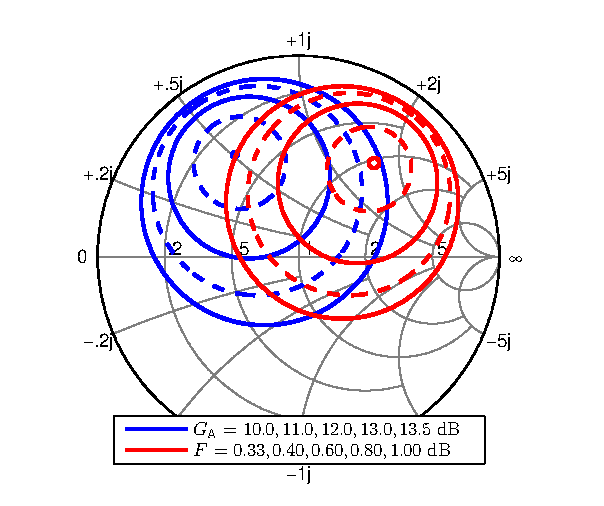
\epsfig{file=img/GFcirc.eps, width=0.6\textwidth}
		\caption{Constant available gain $G_\mathrm{A}$ and noise figure $F$ circles at $f = 2.5$~GHz.}
		\label{f:GFcirc}
	\end{center}
\end{figure}

To meet the return loss specification, $\rho_\mathrm{S}$ must be chose quite close to gain 
maximum. In the pre-design, $\rho_\mathrm{S}$ was chosen with this in mind while the output 
was conjugate-matched. Chosen reflection coefficients and the properties for the pre-design 
are shown if Eq. (\ref{e:Rs}-\ref{e:Rout}) and Table \ref{t:pre2}, respectively. Formulae used 
to find $\mathit{RL}_\mathrm{in}$, $\mathit{RL}_\mathrm{out}$ and $F$ are shown in Eq. (\ref{e:RLin} - \ref{e:F}).
\begin{eqnarray}
\rho_\mathrm{S}		&=\;\;	-0.191 + \mathrm{j} 0.461	\;\;=& 	0.499 \,\angle {+112.6 {\,}^\circ}	\label{e:Rs}	\\
\rho_\mathrm{in}	&=\;\;	-0.307 - \mathrm{j} 0.503	\;\;=& 	0.589 \,\angle {-121.5 {\,}^\circ}	\label{e:Rin}	\\
\rho_\mathrm{L}		&=\;\;	+0.461 + \mathrm{j} 0.171	\;\;=&	0.492 \,\angle {+20.4 {\,}^\circ}	\label{e:Rl}	\\
\rho_\mathrm{out}	&=\;\;	+0.461 - \mathrm{j} 0.171	\;\;=& 	0.492 \,\angle {-20.4 {\,}^\circ}	\label{e:Rout} 
\end{eqnarray}

\begin{table}[!h]
	\begin{center}
		\caption{Properties of the pre-design.}
		\label{t:pre2}
		\renewcommand{\arraystretch}{1.2}
		\begin{tabular}{lccc}
			Parameter						&	Value [dB]	& Design goal [dB] 	& Margin [dB]	\\
			\hline
			$\mathit{RL}_\mathrm{in}$		&	15.22		& $\geq 15$ 		& 0.22			\\
			$\mathit{RL}_\mathrm{out}$		&	$\infty$	& $\geq 15$  		& $\infty$		\\
			$G_\mathrm{A}$					&	13.35		& $\geq 13$  		& 0.35			\\				
			$G_\mathrm{T}$					&	13.35		& $\geq 13$  		& 0.35			\\
			$G_\mathrm{P}$					&	13.49		& $\geq 13$  		& 0.49			\\
			$F$								&	0.737		& $\leq 0.8$ 		& 0.062				
		\end{tabular}
	\end{center}
	\vspace{-1\oneLine}
\end{table}

\begin{eqnarray}
\mathit{RL}_\m{im} 	&=& -10 \lg \left( 1 - \frac{P_\m{in}}{P_\m{avs}} \right) \;\dB \;\;=\;\; -10 \lg \left( 1 - \frac{G_\m{T}}{G_\m{P}} \right) \;\dB \label{e:RLin} \\
\mathit{RL}_\m{out} &=& -10 \lg \left( 1 - \frac{P_\m{L}}{P_\m{avn}} \right) \;\dB \;\;=\;\; -10 \lg \left( 1 - \frac{G_\m{T}}{G_\m{A}} \right) \;\dB \label{e:RLout} \\
F 					&=& 10 \lg \left( F_\m{min} + \frac{4 R_\mathrm{n}}{Z_0} \, \frac{ |\rho_\m{S} - \rho_\m{opt}|^2 }{(1 - |\rho_\m{S}|^2) |1 + \rho_\m{opt}|^2} \right) \;\dB \label{e:F}
\end{eqnarray}

Thus it is in theory possible to achieve all design goals, but only when the transistor 
is stabilized with a suitable series resistor connected to the drain. Increasing this resistance
moves constant gain and noise figure circles close together while decreasing total gain.
Without this resistor the circles are far apart, and the specifications cannot be met. 
Tuning the value of this transistor one may optimize the design for desired characteristics. 
A gain high as 14.7~dB and a noise figure as low as 0.722~dB may be obtained separately, 
when zero-margins are accepted for all other possible criteria.

If this stabilizing resistor cannot be used, one can always resort to balanced amplifiers 
and IDCS designs, but they both have their own drawbacks. In practice the situation will 
be more difficult as any practical realization of DC-biasing will affect the performance 
characteristics.

For simplicity, open parallel stub matching is used to realize both input and output matching 
circuits. Traditional matching process (where one moves toward the generator) may be used, if 
we match the complex conjugates instead the actual values. Thus, the impedances to be matched 
are
\begin{eqnarray}
\rho_\mathrm{S}^* &=\;\; -0.191 - \mathrm{j} 0.461 \;\;=\;\; 0.499 \,\angle {-112.6 {\,}^\circ} 	& \Rightarrow\;\; z_\mathrm{S}^* \;=\; 0.460 - \mathrm{j} 0.565, \\
\rho_\mathrm{L}^* &=\;\; +0.461 - \mathrm{j} 0.171 \;\;=\;\; 0.492 \,\angle {-20.4 {\,}^\circ} 	& \Rightarrow\;\; z_\mathrm{L}^* \;=\; 2.371 - \mathrm{j} 1.070.
\end{eqnarray}
The matching process is shown on the Smith charts in Figures \ref{f:Rs} and \ref{f:Rl}. 
The stub distances/lengths are also shown in Table \ref{t:m2}.

\begin{figure}[!h]
	\begin{center}
		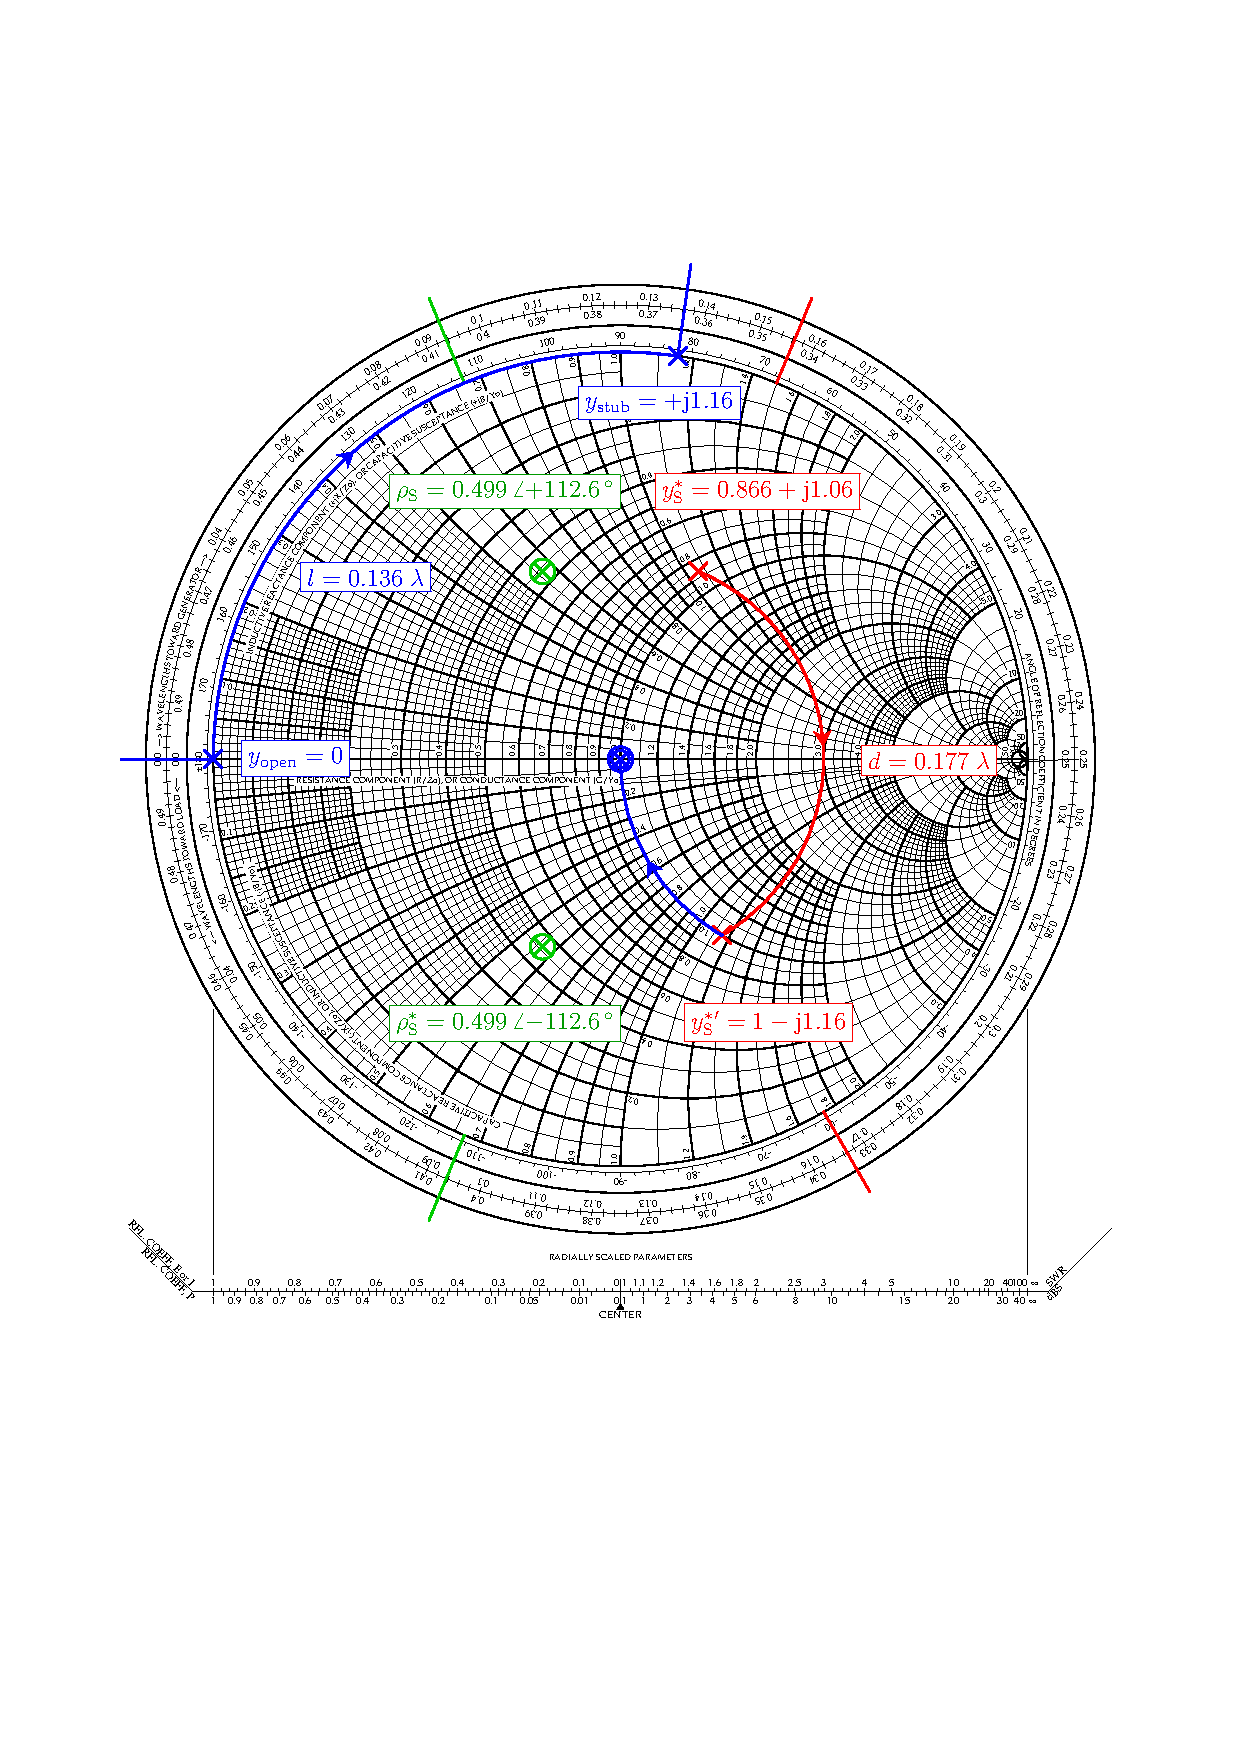
\includegraphics[width=\textwidth]{img/srcSmith.pdf}
		\caption{Input matching circuit using open-circuited parallel stubs.}
		\label{f:Rs}
	\end{center}
\end{figure}

\begin{figure}[!h]
	\begin{center}
		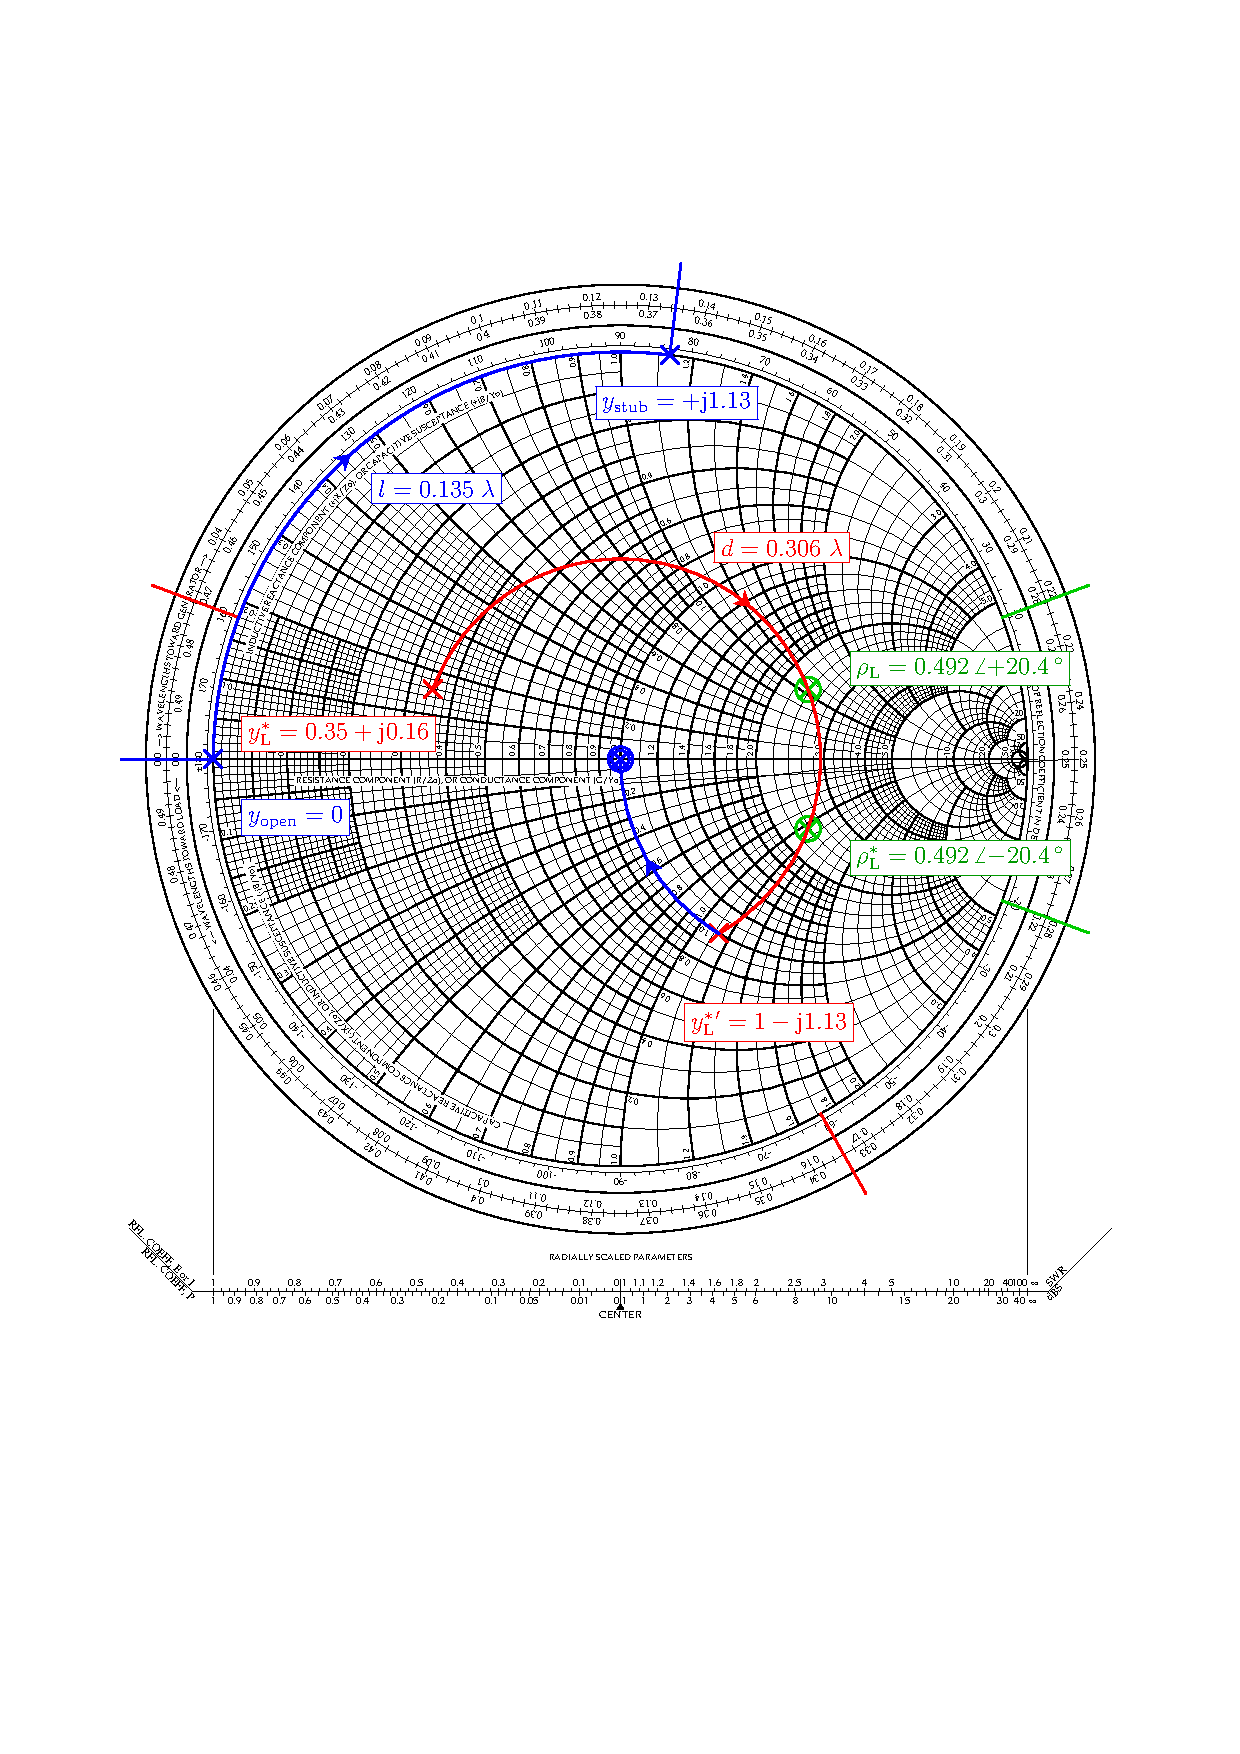
\includegraphics[width=\textwidth]{img/loadSmith.pdf}
		\caption{Output matching circuit using open-circuited parallel stubs.}
		\label{f:Rl}
	\end{center}
\end{figure}

\begin{table}[!h]
	\begin{center}
		\caption{Matching circuits of the pre-design ($Z_0 = 50\;\Omega$).}
		\label{t:m2}
		\renewcommand{\arraystretch}{1.2}
		\begin{tabular}{lccc}
			Port		&	Distance from transistor $d$ [$\lambda$]	& Stub length $l$ [$\lambda$]	\\
			\hline
			Input		&	0.177				& 0.136				\\
			Output		&	0.306				& 0.135			
		\end{tabular}
	\end{center}
	\vspace{-\oneLine}
\end{table}


\newpage
\vspace*{1pt}
\newpage
\subsection{Draw the final schematic of the amplifier including the matching circuits.}

A circuit schematic of the rough pre-design, including stabilization resistor and matching circuits, 
is shown in Fig.~\ref{f:c}.

\begin{figure}[!h]
	\begin{center}
		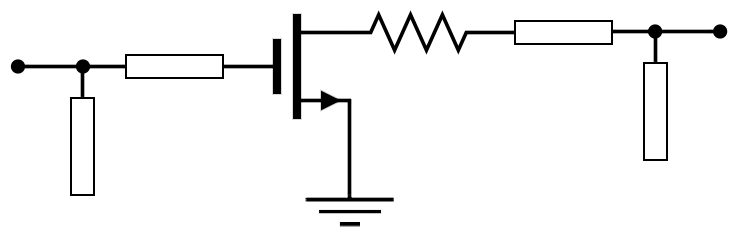
\includegraphics[scale=1]{img/circuit.png}
		\setlength{\unitlength}{1mm}
		\begin{picture}(1,1)
		\linethickness{0.5mm}
		\put(-71, 13.3){\small IN}
		\put(-56.5, 16.7){\small$0.177\;\lambda$}
		\put(-72.5, 6){\small$0.136\;\lambda$}
		\put(-34, 12){\small$100\;\Omega$}
		\put(-23.5, 19.5){\small$0.306\;\lambda$}
		\put(-7, 9){\small$0.135\;\lambda$}
		\put(-1, 16){\small OUT}
		\end{picture}
		\caption{Amplifier pre-design ($Z_0 = 50\;\Omega$).}
		\label{f:c}
	\end{center}
\end{figure}


\newpage
\begin{thebibliography}{9}%\itemsep 7pt\parskip -5pt 
\addcontentsline{toc}{section}{References}

\bibitem{bahl} I.\ J.\ Bahl, 
	\textit{Fundamentals of RF and Microwave Transistor Amplifiers},
	J.\ Wiley \& Sons, 2009.

\bibitem{gonz} G.\ Gonzalez, 
	\textit{Microwave Transistor Amplifiers -- Analysis and Design},
	Prentice Hall, 2nd Ed., 1997.
	
\bibitem{pozar} D.\ M.\ Pozar, 
	\textit{Microwave Engineering}, 
	J.\ Wiley \& Sons, 4th Ed., 2012.

\end{thebibliography}

\newpage
\section*{Appendix A: MATLAB source code}
\addcontentsline{toc}{section}{Appendix A: MATLAB source code}

The source code MATLAB script used in the pre-design process is shown below. 
Apart from \texttt{exportfig}, all other features are self-made. No RF 
toolbox is required, meaning the script might also be compatible with GNU Octave.

\lstinputlisting[language=Matlab]{src/p4.m}


\end{document}
